Chapter \ref{s:definitions-types} on page \pageref{s:definitions-types} already defines \ac{GeoVis}. It is closely related to \ac{InfoVis} and \ac{SciVis} and emphazises knowledge construction over knowledge storage or information transmission \iacite{maceachren:1997}. Owing to its roots in cartography, \ac{GeoVis} contributes to its related fields by way of the map metaphor, which "[\ldots] has been widely used to visualize non-geographic information in the domains of information visualization and domain knowledge visualization" \iacite{Jiang2005}.
In short, the thesis uses the term \ac{GeoVis} as a hypernym for the combination of exploratory data analysis, \ac{InfoVis}, \ac{SciVis}, thematic cartography and visual analytics.

\ac{GeoVis} are superior to traditional, static maps because they are not limited to exploration capabilities. They allow more interaction in maps, due to the ability of extending the basic layer of the map with user-experience abilities like zooming to change the visual appearance \iacite{Jiang2003}. These kinds of visualizations are also used in practical applications which are briefly outlined in this chapter.

\begin{description}

\item[Urban Planning] \hfill \\
Urbanists use \ac{GeoVis} to "[\ldots] model environmental interests and policy concerns of the general public" \iacite{Jiang2003}. \citeauthor{Jiang2003} also mention two examples, in which "[\ldots] 3D photorealistic representations are used to show urban redevelopment and dynamic computer simulations are used to show possible pollution diffusion over the next few years".
\citeauthor{Jiang2003} also describe that the widespread use of the internet by the general public impacts collaborative planning. The former way of planning in committee rooms or computer facility rooms can now be extended with a decentralised web platform. The use of the internet features two important aspects of planning:
\begin{enumerate*}
\item it already integrates various interactive and proactive techniques and
\item it is time and place independent.
\end{enumerate*}

\item[Environmental Studies] \hfill \\
\citeauthor{Danado2005} describe a system that is capable of simulating and visualizing environmental processes collaboratively. In addition, the system has the ability to retrieve information while moving in real time. Thus each user can impact the simulation by adding or removing information to or from the model. The system also reacts on the changes the users made, therefore making it possible to explore a complex set of environmental data, affecting it with different actions and determine a best fit \iacite{Danado2005}.

\item[Forestry] \hfill \\
\citeauthor{Andrienko2007} present a system to visualize a large set of spatio-temporal data related to european forests. The innovative approach of this system is given by the interaction. Non-experts can change parameters in the system and explore the results. Furthermore \citeauthor{Andrienko2007} state their approach "[\ldots] uncovers a range of fundamental issues relevant to the broad field of \ac{GeoVis} and \ac{InfoVis} research \iacite{Andrienko2007}."

\citeauthor{Andrienko2007} also cited the two major problems as
\begin{enumerate}
\item the inability of the geovisualizers to convince the foresters of the efficiency of \ac{GeoVis} in their work and
\item the foresters' misgivings over the dataset's accessibility to non-experts engaging in "uncontrolled exploration".
\end{enumerate}

\item[Telecommunication] \hfill \\
\ac{GeoVis} are also very helpful in the area of telecommunication. Telegeography\footnote{https://www.telegeography.com/}, as an example for a company in that specific area, has an interactive submarine cable map. Figure \ref{fig:both-submarines} on page \pageref{fig:both-submarines} features an overview of this map (see figure \ref{fig:submarine}) and the interactivity (see figure \ref{fig:submarine-interactive}) which gives more information to the cable’s profile, including the cable’s name, ready-for-service date, length, owners, website, and landing points.

\begin{figure}[!htb]
  \captionsetup[subfigure]{justification=centering}
  \centering
  \begin{subfigure}[b]{0.4\textwidth}
    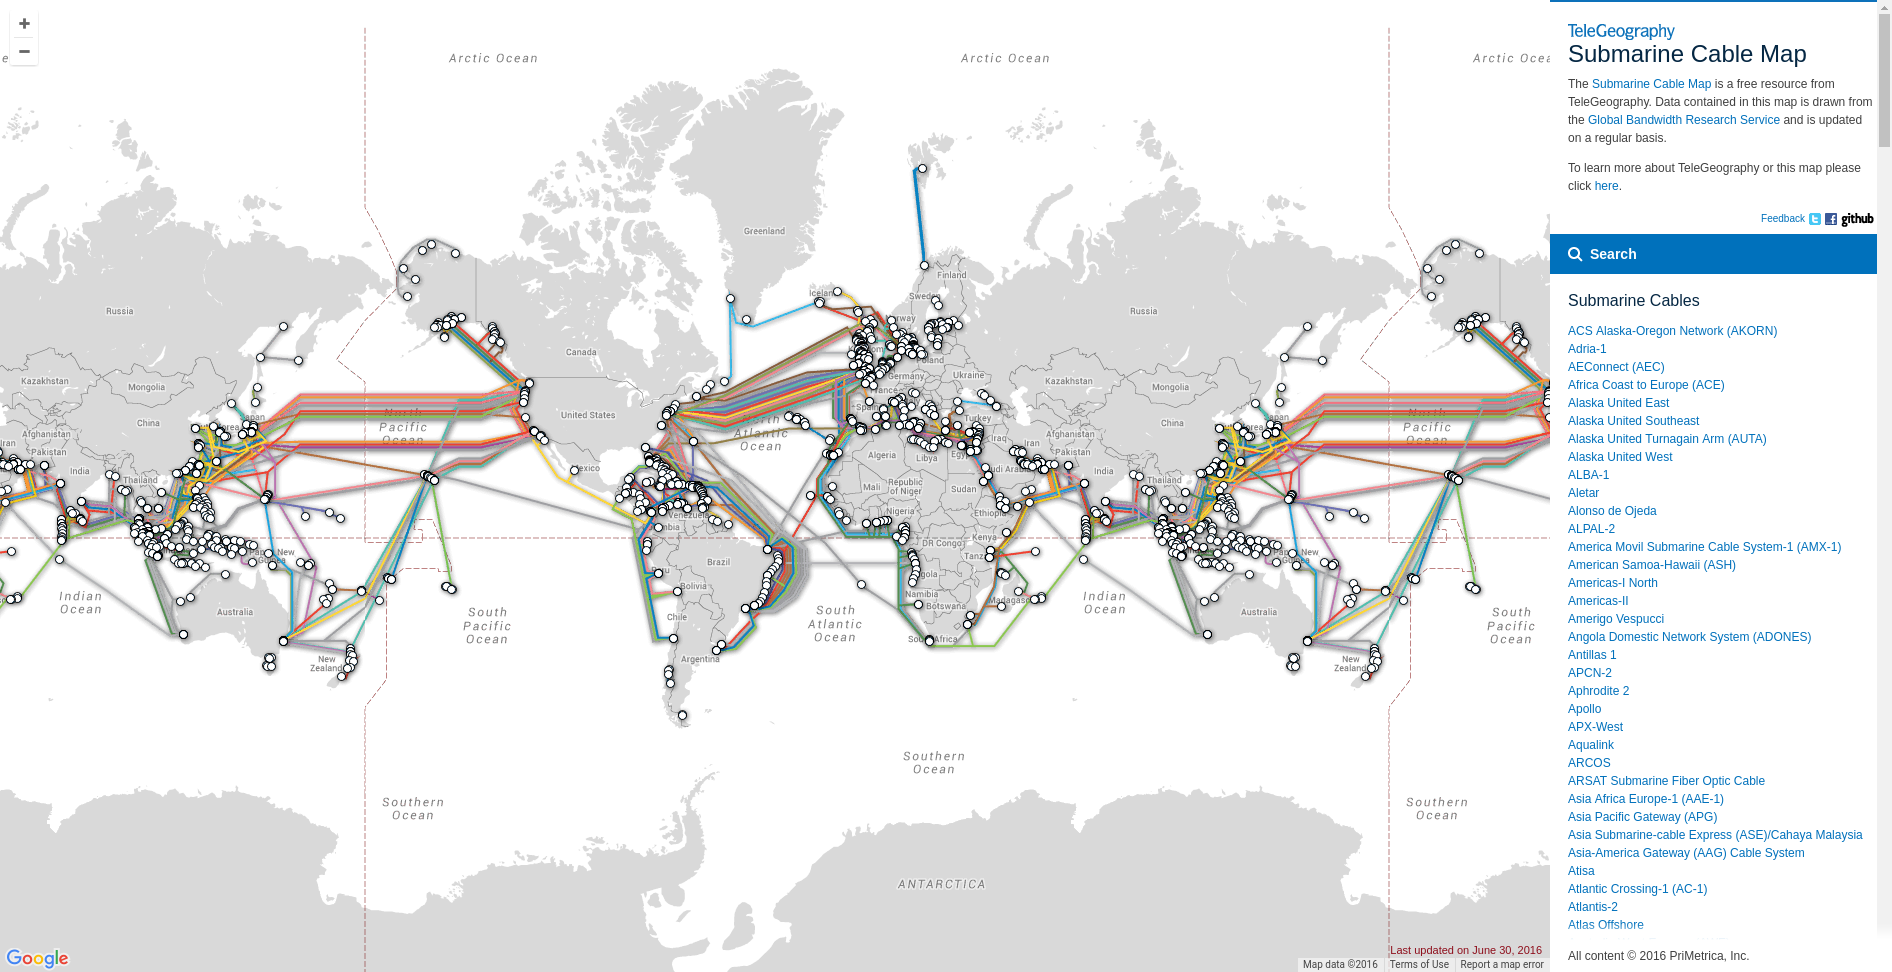
\includegraphics[width=\textwidth]{images/geovis/submarine.png}
    \caption[Overview of the submarine cable map]{Overview of the submarine cable map}
    \label{fig:submarine}
  \end{subfigure}
  \hfill
  \begin{subfigure}[b]{0.4\textwidth}
    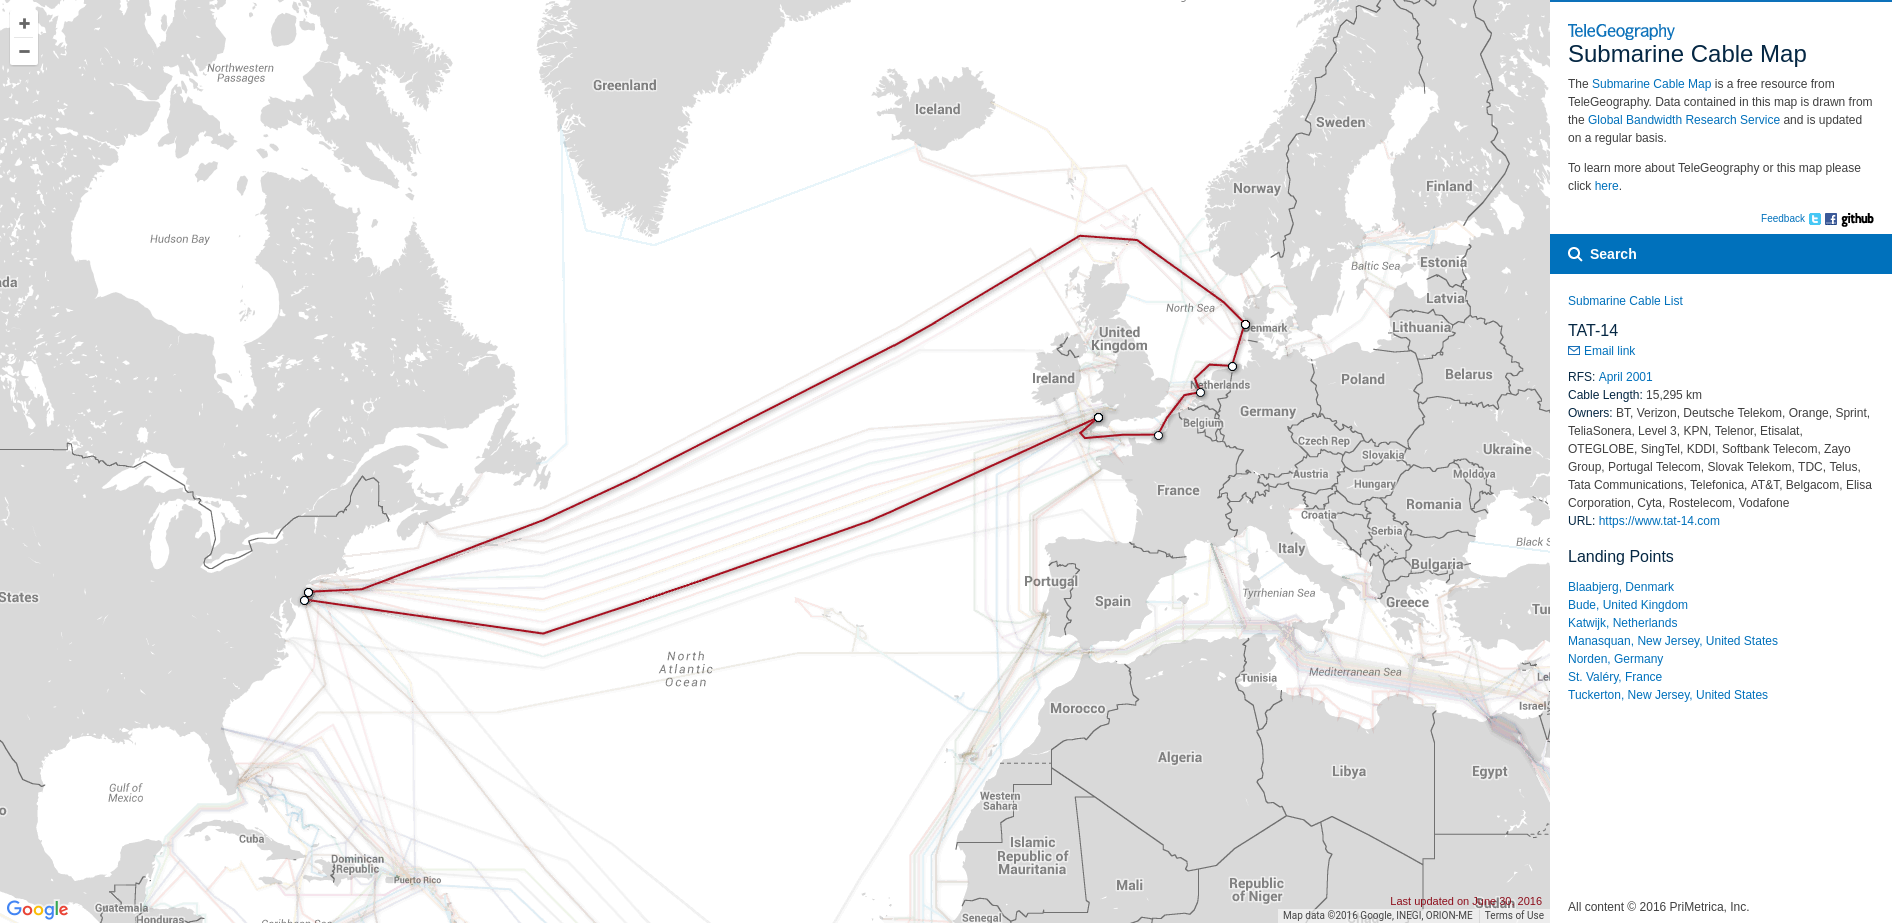
\includegraphics[width=\textwidth]{images/geovis/submarine-interactive.png}
    \caption[Interactivity of the submarine cable map]{Interactivity of the submarine cable map}
    \label{fig:submarine-interactive}
  \end{subfigure}
    \caption[
        TeleGeography’s free interactive submarine cable map, Urldate: 07.2016 \newline
    \small\texttt{\url{http://www.submarinecablemap.com/}}
    ]{TeleGeography’s free interactive submarine cable map}
  \label{fig:both-submarines}
\end{figure}

\item[E-commerce] \hfill \\
\ac{GeoVis} can be very useful in analysing data provided by e-commerce shops if they track orders-behaviour of their customers with some kind of geographical information. If such data is available and provided, it is possible to easily visualize the target group of a company on a map and therefore create knowledge and allow for generating hypothesis i.e. the next region for expansion.

\end{description}